%%
%% This is file `sample-sigconf.tex',
%% generated with the docstrip utility.
%%
%% The original source files were:
%%
%% samples.dtx  (with options: `sigconf')
%% 
%% IMPORTANT NOTICE:
%% 
%% For the copyright see the source file.
%% 
%% Any modified versions of this file must be renamed
%% with new filenames distinct from sample-sigconf.tex.
%% 
%% For distribution of the original source see the terms
%% for copying and modification in the file samples.dtx.
%% 
%% This generated file may be distributed as long as the
%% original source files, as listed above, are part of the
%% same distribution. (The sources need not necessarily be
%% in the same archive or directory.)
%%
%% The first command in your LaTeX source must be the \documentclass command.
\documentclass[sigconf]{acmart}

%%%% As of March 2017, [siggraph] is no longer used. Please use sigconf (above) for SIGGRAPH conferences.

%%%% As of May 2020, [sigchi] and [sigchi-a] are no longer used. Please use sigconf (above) for SIGCHI conferences.

%%%% Proceedings format for SIGPLAN conferences 
% \documentclass[sigplan, anonymous, review]{acmart}

%%%% Proceedings format for conferences using one-column small layout
% \documentclass[acmsmall,review]{acmart}

%%
%% \BibTeX command to typeset BibTeX logo in the docs
\AtBeginDocument{%
  \providecommand\BibTeX{{%
    \normalfont B\kern-0.5em{\scshape i\kern-0.25em b}\kern-0.8em\TeX}}}

%% Rights management information.  This information is sent to you
%% when you complete the rights form.  These commands have SAMPLE
%% values in them; it is your responsibility as an author to replace
%% the commands and values with those provided to you when you
%% complete the rights form.
\setcopyright{acmcopyright}
\copyrightyear{2018}
\acmYear{2018}
\acmDOI{10.1145/1122445.1122456}

%% These commands are for a PROCEEDINGS abstract or paper.
\acmConference[Woodstock '18]{Woodstock '18: ACM Symposium on Neural
  Gaze Detection}{June 03--05, 2018}{Woodstock, NY}
\acmBooktitle{Woodstock '18: ACM Symposium on Neural Gaze Detection,
  June 03--05, 2018, Woodstock, NY}
\acmPrice{15.00}
\acmISBN{978-1-4503-XXXX-X/18/06}


%%
%% Submission ID.
%% Use this when submitting an article to a sponsored event. You'll
%% receive a unique submission ID from the organizers
%% of the event, and this ID should be used as the parameter to this command.
%%\acmSubmissionID{123-A56-BU3}

%%
%% The majority of ACM publications use numbered citations and
%% references.  The command \citestyle{authoryear} switches to the
%% "author year" style.
%%
%% If you are preparing content for an event
%% sponsored by ACM SIGGRAPH, you must use the "author year" style of
%% citations and references.
%% Uncommenting
%% the next command will enable that style.
%%\citestyle{acmauthoryear}

%%
%% end of the preamble, start of the body of the document source.
\begin{document}

%%
%% The "title" command has an optional parameter,
%% allowing the author to define a "short title" to be used in page headers.
\title{Forexast: A Interactive News Digestion for Forex Investors}

%%
%% The "author" command and its associated commands are used to define
%% the authors and their affiliations.
%% Of note is the shared affiliation of the first two authors, and the
%% "authornote" and "authornotemark" commands
%% used to denote shared contribution to the research.
\author{Ben Trovato}
\authornote{Both authors contributed equally to this research.}
\email{trovato@corporation.com}
\orcid{1234-5678-9012}
\author{G.K.M. Tobin}
\authornotemark[1]
\email{webmaster@marysville-ohio.com}
\affiliation{%
  \institution{Institute for Clarity in Documentation}
  \streetaddress{P.O. Box 1212}
  \city{Dublin}
  \state{Ohio}
  \postcode{43017-6221}
}



\author{Huifen Chan}
\affiliation{%
  \institution{Tsinghua University}
  \streetaddress{30 Shuangqing Rd}
  \city{Haidian Qu}
  \state{Beijing Shi}
  \country{China}}

\author{Charles Palmer}
\affiliation{%
  \institution{Palmer Research Laboratories}
  \streetaddress{8600 Datapoint Drive}
  \city{San Antonio}
  \state{Texas}
  \postcode{78229}}
\email{cpalmer@prl.com}


%%
%% By default, the full list of authors will be used in the page
%% headers. Often, this list is too long, and will overlap
%% other information printed in the page headers. This command allows
%% the author to define a more concise list
%% of authors' names for this purpose.
\renewcommand{\shortauthors}{Trovato and Tobin, et al.}

%%
%% The abstract is a short summary of the work to be presented in the
%% article.
\begin{abstract}
Foreign exchange (forex) markets reflect real-world events, local or global.  Thus,  financial news is oftentimes referred to when making predicting the trends of forex. We propose News Forexast,  an interactive web-based system that displays a forex plot alongside with related financial news. Users can locate specific periods when the trading trends in forex markets dramatically change with the visualization of Standard Deviation (SD) events and Directional Change (DC) events. Finally, Forex comes with a keyword filtering function that allows users to filter news with keywords. We aim to make the decision-making process smoother for not only professional financial analysts but also all investors with this accessible and intuitive website.
\end{abstract}

%%
%% The code below is generated by the tool at http://dl.acm.org/ccs.cfm.
%% Please copy and paste the code instead of the example below.
%%
\begin{CCSXML}
<ccs2012>
   <concept>
       <concept_id>10002951.10003260.10003282</concept_id>
       <concept_desc>Information systems~Web applications</concept_desc>
       <concept_significance>500</concept_significance>
       </concept>
 </ccs2012>
\end{CCSXML}

\ccsdesc[500]{Information systems~Web applications}


%%
%% Keywords. The author(s) should pick words that accurately describe
%% the work being presented. Separate the keywords with commas.
\keywords{forex, financial news, standard deviation, directional change}

%% A "teaser" image appears between the author and affiliation
%% information and the body of the document, and typically spans the
%% page.
\begin{teaserfigure}
  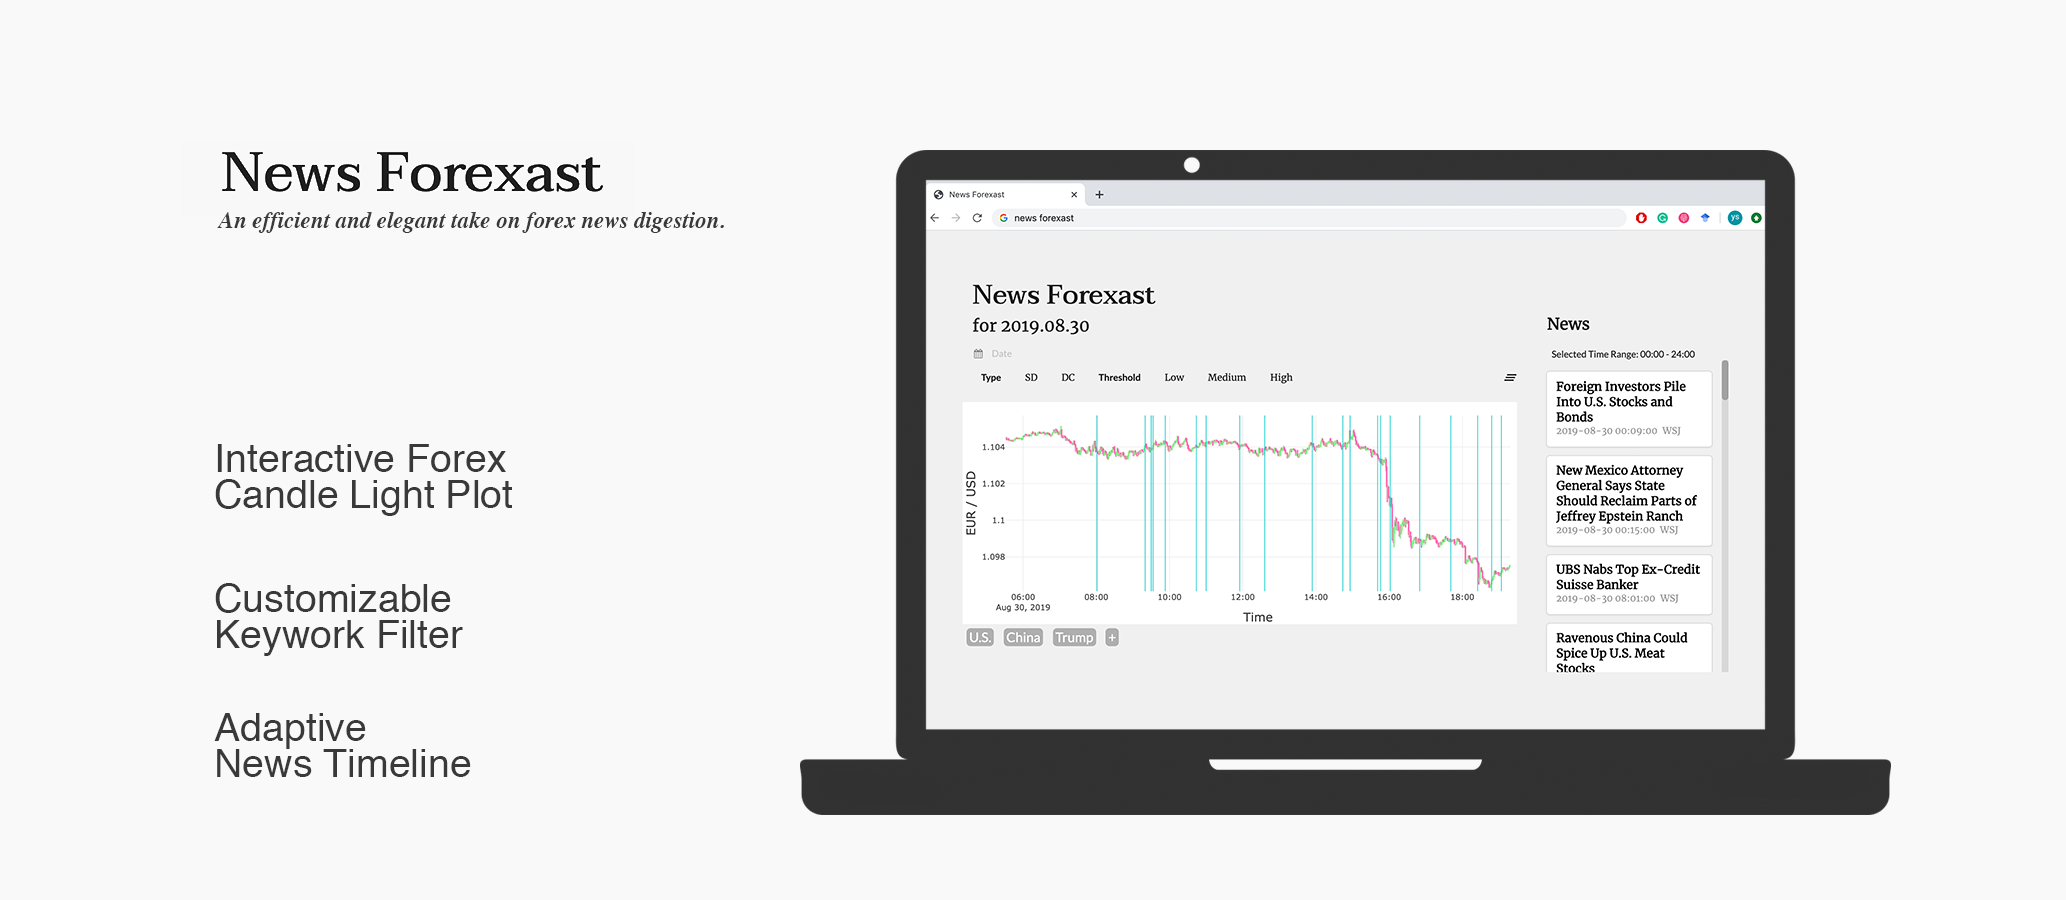
\includegraphics[width=\textwidth]{teaser.png}
  \caption{Forexast available at http://}
  \Description{}
  \label{fig:teaser}
\end{teaserfigure}


%%
%% This command processes the author and affiliation and title
%% information and builds the first part of the formatted document.
\maketitle

\section{Introduction}
Foreign exchange (Forex) market has been one of the most popular market for decades, with an estimated \$1\  trillion traded every day\cite{YAO200079}. Spot trading, options future and exchange-traded funds(ETFs) are three of many ways of investing strategies adopted in forex markets\cite{TradeForex}. The strategies might vary but they are driven by an intuitive rule of thumb, which is to buy low and sell high\cite{KOOLEN2014144}\cite{Zervos11}. Therefore, whether investors can accurately forecast the prices or trends is extremely crucial. Forex markets are influenced by numerous factors, such as producer price index(PPI), interest rates and politics, in order to consider as many factors as possible to have more comprehensive approaches for forex investment, investors rely on news for them to stay informed. Besides the fact that news usually reflect the real world events, the similar nature of news and forex also makes these two co-dependent. For example, if the Federal Reserve System (Fed) cuts the interest rate, it is more likely that the value of USD would drop, the devaluation would then feed into forex market increasing the demand, thus making another piece of news. 

\section{Related Work and Systems}
The dynamics between news and forex markets have been explored from several different aspects. Evans and Lyons proved that news can have significant effects on currency for days\cite{EVANS2005197}, and more specifically macro news can affect currency prices directly and indirectly via order flow\cite{EVANS200826}. There is also more evidence showcasing news and forex trend are correlated, Bauwens, Omrane and Giot show that volatility increases right before the announcement of scheduled news and unscheduled-but-periodic news\cite{BAUWENS20051108}, while Chatrath et al. suggests that prices respond quickly within 5-min of the news release\cite{CHATRATH201442}. With how forex markets and news interact in mind, it is only reasonable to suggest traders should begin their days by reading news commentary to determine the market sentiment and the daily direction for trading\cite{samuels2015trader}.

There are many trading websites which provide useful information for forex investors, and each of them has its own features\cite{ForexWebsites}. For instance, BabyPips\cite{BabyPips} is a friendly website for junior traders, which provides not only forex plots and data but also courses, tutorials and forums for beginners. Bloomberg\cite{Bloomberg} is a well-known news agency. Therefore, besides stocks and currencies data, it also has various categories of news. TradingView\cite{TradingView} provides numerous functions in a page, such as watchlist, alerts, headlines and real-time chats, where users can customize the settings. However, some of their news and forex plot are not put in the same interface, or the times of news and forex are not highlighted. This could neglect the relation between news and forex data. Therefore, our work aims to highlight the connection between the timing of news and forex trends. New Forexast is designed to display the news’ release time as vertical lines on the forex plot to emphasize the order of breaking news and exchange rates. In addition, when users hover on the line, the background colour of the corresponding news would change. 
We also choose to display standard deviation events (SD events) and directional change events (DC events)\cite{7850020} to help users locate the changes within exchange rates, and pay more attention to the changes of trend or where the prices have larger volatility. The features of News Forexast would be introduced more detailed in section 4.




\section{System Structure}

\subsection{Data Collection}
The forex data is from philipperemy/FX-1-Minute-Data\cite{FX-1-Minute-Data}, a repository of github. We choose the EUR/USD index, and use the DateTime Stamp, OPEN Bid Quote, HIGH Bid Quote, LOW Bid Quote and CLOSE Bid Quote columns as our forex data. The time span is from 2019/08/04 to 2019/09/13 except Saturdays, and the granularity of data is minute. 

The news data is crawled by us, containing titles, sources, release times and urls. There are 1116 news in total and the sources are all from The Wall Street Journal\cite{WSJ}.

\subsection{Algorithms for DC and SC events}
To mark some special time points on the plot, we use two algorithms, standard deviation events (SD events) and directional change events (DC events)\cite{7850020}. SD events show the times where the prices dramatically change, and DC events show the times where the trends change. To get these events, we need to calculate the difference rate list $D$ of the price list first. 
Let $P= [p_1, p_2, ..., p_n]$, where $p_t$ stands for the CLOSE Bid Quote at minute $t$ and n equals to total numbers of daily forex data. Then we can get a difference rate list $D= [d_1, d_2, ..., d_m]$, where $d_t = \frac{p_{t+w}-p_t}{p_t}$.  $w\in\mathbb Z^+$ means the range in minutes, which can be freely customized (we use 30 in this demonstration).
$\sigma$ is the standard deviation of $D$, which can be interpreted as the volatility of prices. We use $\sigma$ as our low threshold to attain a subset of D, whose elements are all bigger than $\sigma$. Then the corresponding set of p will be marked as SD events. We also consider $2\sigma$ and $3\sigma$ as medium and high thresholds in our demonstration. Higher threshold will find less events.

Under the DC framework, the market is summarized into alternating uptrends and downtrends\cite{7850020}. A DC event, including a start point and an end point, can be seen as a period that the trend starts to change. At first, we do not know the prices start with a upward or downward trend, so we let the first element of price $p_1$ as a base. Then we start looking through the list until we find a current price $p_c$, where $|\frac{p_c-p_1}{p_1}| > \theta$, $\theta$ can be set to $\sigma$, $2\sigma$, $3\sigma$ as above mentioned. If $p_c > p_1$, that means the span from $p_1$ to $p_c$ is an upward DC event; otherwise, it is a downward DC event. After finding the first DC event, we still have to look through the rest. Let us consider a market starts with a downtrend, which means we are now in an downtrend and waiting for a next uptrend. We keep updating the lowest price $p_l$ in this downtrend until we find a current price $p_c$ that $\frac{p_c-p_l}{p_l} > \theta$. Then, we mark that the span from $p_l$ to $p_c$ is a upward DC event, and the trend become upward. Similarly, if a market is in a uptrend, we keep updating the highest price $p_h$ until we find a current $p_c$ that $\frac{p_h-p_c}{p_c} > \theta$, then $p_h$ to $p_c$ is a downward DC event, and the trend become downward. After finishing looking through all daily forex data, we can get a series of alternating DC events.




\section{Interfaces and features}
The interface of News Forexast can be divided into two main parts, a forex chart and the news section. Users can customize the selection criteria either by directly manipulating the forex chart or applying the keyword filters.

\begin{figure}[h]
  \centering
  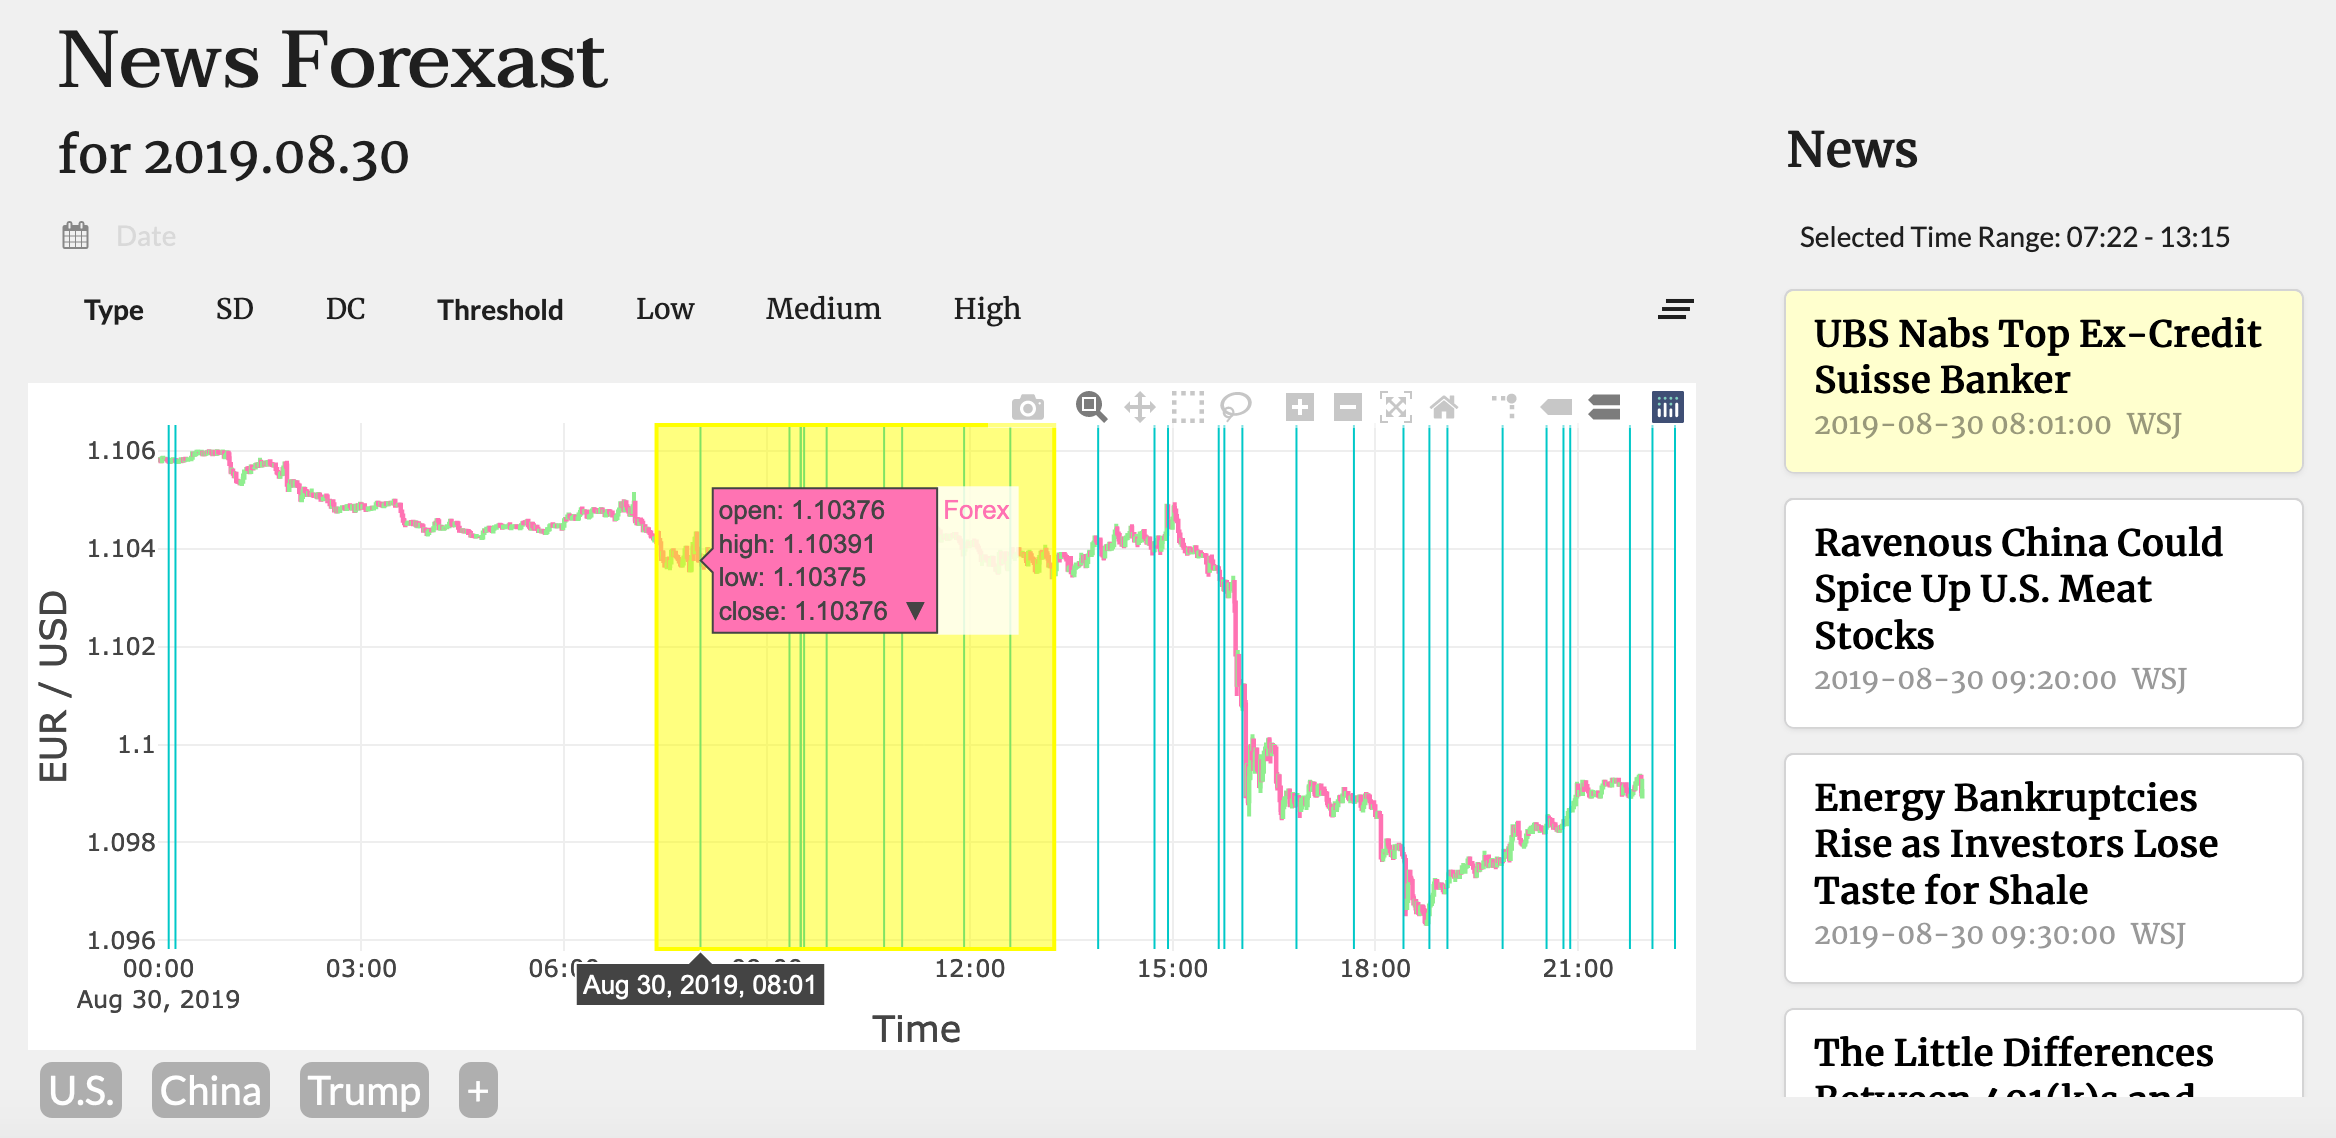
\includegraphics[width=\linewidth]{hover.png}
  \caption{Example of news being highlighted when the cursor hovers over the corresponding timeline on the chart.}
  \Description{}
\end{figure}

\subsection{Interactive Forex Chart}
The forex chart is a standard candlestick chart, powered by Plotly graphing libraries\cite{Plotly}, that displays price movements, users can specify the date they are interested in with the calendar icon above the chart. Supported by Plotly graphing library, users can explore the chart freely by zooming in or dragging out the time frame they are interested. The corresponding news would be highlighted if users hover over the corresponding blue line on the chart. (Fig. 2)


Below the calendar is where users can specify event types and the corresponding thresholds. After selecting an event type and their thresholds, eg. SD and low threshold,  the algorithmic output would be shown on the forex chart. Once done with a specific setting, users can clear the setting with the “clear all” button the top-right. The news section without any specification would show all daily news with titles, released time and sources. Users could link to the original posts and websites by clicking on the news cards. 



\subsection{Forex Event Identifier}
With the help of SD and DC events as indicators, users can now spot specific time ranges they are interested in. (Fig 3, 4) Users can then select such time range on the plot and narrow down the news shown on the right to the time range they selected. For example, users can specify 2019/08/30 with the SD with the low threshold, users can tell that there’s a dramatic change during 14:30-16:30 and can proceed to select the time range on the plot. In return, the news section would display related news such as "Would Warren Buffett Buy Greenland?" and "Risky Seller Financing Flourishes Where Homes Are Cheapest". 

\begin{figure}[h]
  \centering
  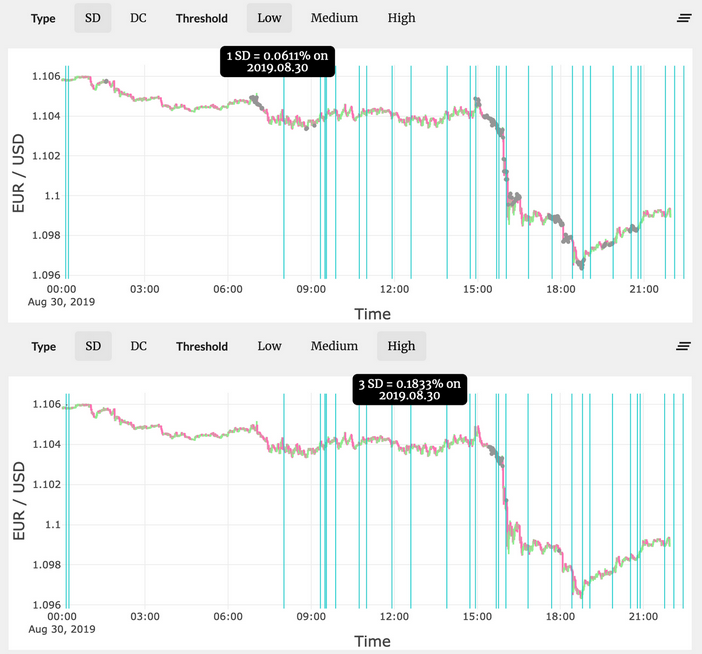
\includegraphics[width=\linewidth]{sd.png}
  \caption{Examples of displaying SD events on 2019/08/30. The top is set to low threshold and the bottom is set to high threshold. Due to the higher sensitivity, almost all events of the latter are in the slump period around 16:00.}
  \Description{}
\end{figure}

\begin{figure}[h]
  \centering
  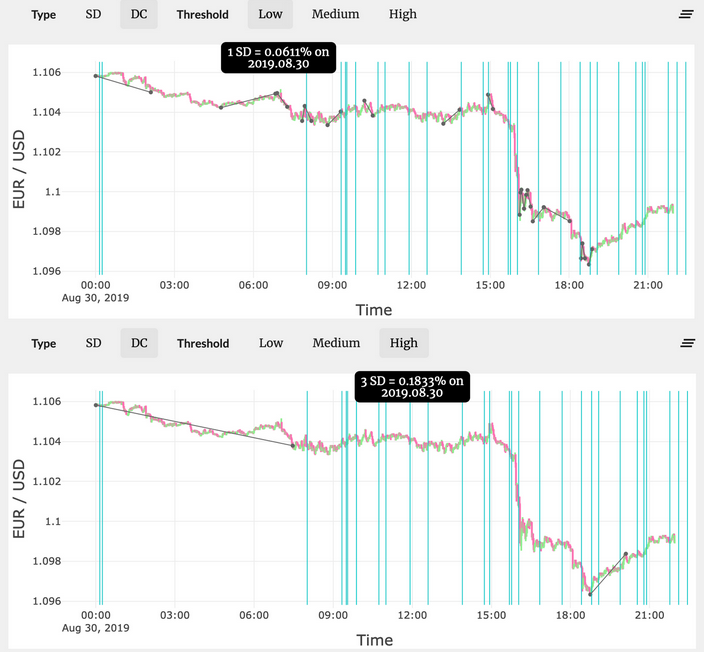
\includegraphics[width=\linewidth]{dc.png}
  \caption{Examples of displaying DC events on 2019/08/30. The top is set to low threshold and the bottom is set to high threshold. Due to the higher sensitivity, the latter only summarize the daily market into a downtrend and an uptrend.}
  \Description{}
\end{figure}

\subsection{Customizable Keyword Filter
}
If interested in more specific news, users can use the button under the plot to filter out news with selected keywords. We have placed several keywords such as U.S. and Trump, users can also customize their own tags by clicking the “+” button. For example, if the time frame is specified and the tag "U.S" is applied, only "Strength in U.S. Consumer Spending Drives Economy". would be shown on the news section.(Fig 5)


\begin{figure}[h]
  \centering
  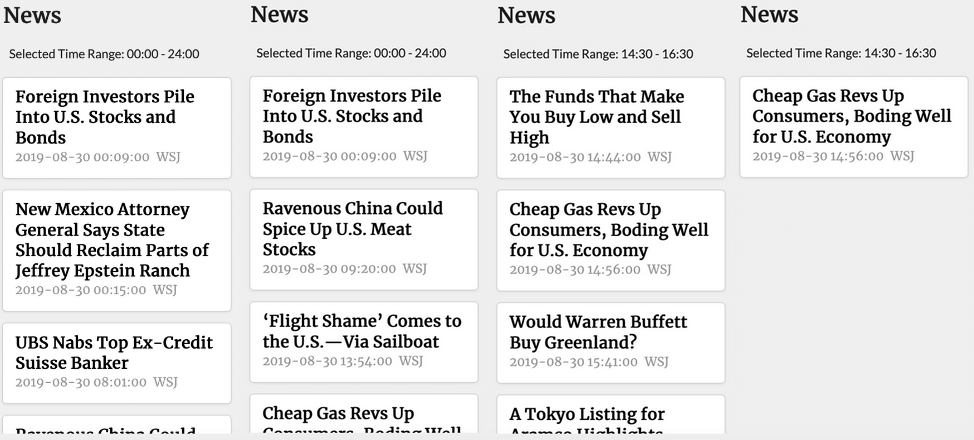
\includegraphics[width=\linewidth]{news.png}
  \caption{Examples of filtering news on 2019/08/30. From left to right are none, keyword: 'U.S.', time: '14:30-16:30', and both.}
  \Description{}
\end{figure}


\section{Conclusion and Future work}
We have proposed an interactive website that juxtaposes a forex chart with news within the time frame users selecting. By having the chart and related news side by side together, users, financial professional or amateur investors, can all understand the trend quicker and easier. We are working toward to provide real-time news update in the future, as fixed data is limited. In addition, if we are able to collect more user's log data and news in the future, along with machine learning and natural language processing (NLP) techniques, we can achieve more customized news feed such as personal news recommendation.  

\section{Acknowledgments}



\bibliographystyle{ACM-Reference-Format}
\bibliography{reference}




\end{document}
\endinput
%%
%% End of file `sample-sigconf.tex'.
